\section{改进方法}

\begin{frame}{改进思路：消去冗余的边界候选}
将覆盖外端点与核心相连的邻居集合称为\textbf{查询边界}。如果一个邻居可达的目标已被另一个邻居覆盖，就可以减少一次候选枚举。
\par\vspace{2mm}
\begin{columns}[c,onlytextwidth]
\column{.54\textwidth}\centering
\resizebox{\linewidth}{!}{
\begin{tikzpicture}[x=10mm,y=5.5mm,
v/.style={circle,draw=Gold,fill=Gold!12,minimum size=7mm,inner sep=0pt,font=\normalsize},
a/.style={-{Stealth[length=2mm]},line width=1pt}]
\node[circle,draw=Line,fill=white,minimum size=7mm](s)at(0,0){$s$};
\node[v](x)at(2,1){$x$};\node[v,draw=Alert,dashed](y)at(2,-1){$y$};
\draw[a,Teal](s)--(x);\draw[a,Edge,dashed](s)--(y);
\filldraw[fill=Teal!7,draw=Teal,rounded corners=2pt](3.8,.45)rectangle(7.1,1.55);
\filldraw[fill=Light,draw=Edge,rounded corners=2pt](3.8,-1.55)rectangle(6.0,-.45);
\foreach \xx/\tt in {4.4/p,5.5/q,6.6/r}{\node at(\xx,1){$\tt$};}
\foreach \xx/\tt in {4.4/p,5.5/q}{\node at(\xx,-1){$\tt$};}
\draw[a,Teal](x)--(3.7,1);\draw[a,Edge](y)--(3.7,-1);
\node[font=\small,Teal]at(5.4,2){$R_b(x)$};
\node[font=\small,Muted]at(4.9,-2){$R_b(y)$};
\end{tikzpicture}}
\column{.43\textwidth}
\begin{block}{阈值支配}
$R_b(u)$ 表示 $u$ 在预算 $b$ 内可达的核心节点集。若
\[
R_b(y)\subseteq R_b(x),
\]
则 $y$ 可由 $x$ 替代。
\end{block}
\end{columns}
\par\vspace{2mm}
出边界比较后继集合，入边界比较前驱集合；约简后仍按原文四类规则完成查询。
\end{frame}

\begin{frame}{关键技术：区分跳数预算与边界方向}
\framesubtitle{$k=3$ 的示例：在论文图中增加一条 $c\to d$}
\begin{columns}[c,onlytextwidth]
\column{.52\textwidth}\centering
\resizebox{\linewidth}{!}{\DominanceGraph{c/b}}\par\vspace{1mm}
\Micro{新增边用青色标记，$N^+(c)=\{b,d\}$。}
\column{.45\textwidth}
{\fontsize{11}{13}\selectfont\setlength{\tabcolsep}{3pt}
\begin{tabular}{@{}cllc@{}}\toprule
预算 & $R(b)$ & $R(d)$ & 保留\\\midrule
1 & $\{b,d\}$ & $\{d\}$ & $b$\\[1mm]
2 & $\{b,d\}$ & $\{b,d,g\}$ & $d$\\\bottomrule
\end{tabular}}\par\vspace{1mm}
\fontsize{11}{13}\selectfont
$c\to g$ 属于第三类查询，预算为 2，需保留 $d$；沿用预算 1 的代表 $b$ 会漏判。
\end{columns}
\begin{block}{实现框架}
离线保存两个预算、两个方向的约简边界；在线按查询类别选取相应列表。
\end{block}
\end{frame}

\section{实验结果}
\begin{frame}{实验设置}
\begin{columns}[T,onlytextwidth]
\column{.49\textwidth}
\begin{tabular}{@{}lrr@{}}\toprule
有向图 & 节点 & 边\\\midrule
Wiki-Vote & 7,115 & 103,689\\
Gnutella31 & 62,586 & 147,892\\
Email-EuAll & 265,214 & 418,956\\\bottomrule
\end{tabular}\par\vspace{3mm}
$k=2,4,6$，主结果取 $k=4$。\par
均匀查询、正负平衡查询。\par
每批 5,000 条，3 个随机种子。
\column{.46\textwidth}
\textbf{对比方案}\par\vspace{1mm}
\begin{itemize}
\item 原始边界：CSR、混合编码、有序表求交。
\item 改进：将双侧支配剪枝与上述表示结合。
\item 消融：仅约简出边界或入边界。
\end{itemize}
\end{columns}
\par\vspace{2mm}
共比较 8 种方案，每种重复计时 9 次。所有查询结果与完整 BFS 一致。
\end{frame}

\begin{frame}{核心查找次数与消融结果}
\framesubtitle{Wiki-Vote，$k=4$，正负平衡查询}
\centering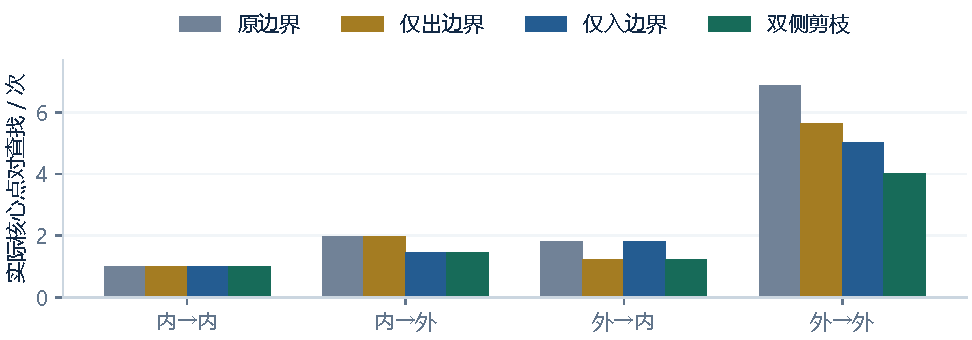
\includegraphics[width=.97\textwidth,height=44mm,keepaspectratio]{case_probes.pdf}\par
{\fontsize{11}{13}\selectfont 双侧剪枝将平均核心查找由 2.01 次降至 1.43 次，减少 29\%。\par 两端均在覆盖内时，查找过程保持不变。}
\end{frame}

\begin{frame}{查询性能与额外开销}
\framesubtitle{$k=4$，在相同混合编码下比较剪枝前后}
\centering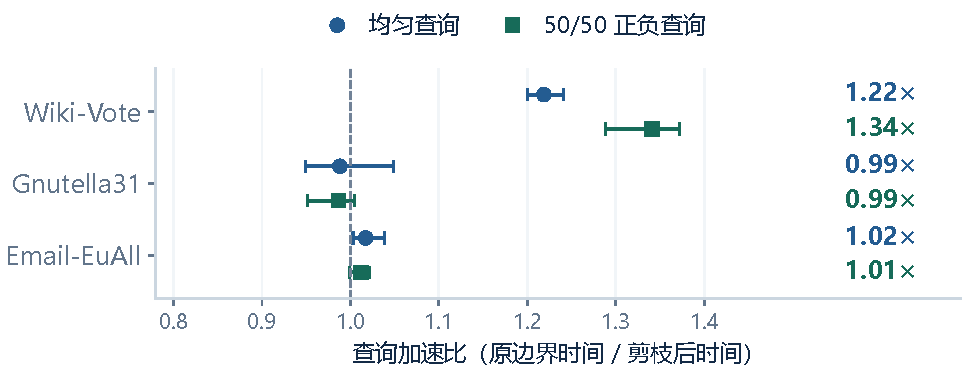
\includegraphics[width=.97\textwidth,height=44mm,keepaspectratio]{pruning_speed.pdf}\par
{\fontsize{11}{13}\selectfont Wiki 上平均加速 1.28 倍；P2P 和 Email 的查询时间变化较小。\par Wiki 增加约 70 KiB 边界索引，构建约 0.10s。}
\end{frame}

\section{总结}
\begin{frame}{总结与创新点}
\begin{columns}[T,onlytextwidth]
\column{.47\textwidth}
\begin{block}{论文的主要贡献}
用顶点覆盖连接任意查询端点，以三档距离信息支持四类精确查询，在索引规模和查询效率之间取得平衡。
\end{block}
\column{.47\textwidth}
\begin{block}{我们的改进}
按有限跳数下的集合支配约简查询边界，为两个预算、两个方向分别保存代表，并通过见证替代保持精确判定。
\end{block}
\end{columns}
\par\vspace{3mm}
实验表明，该方法在冗余边界较多的 Wiki 上减少了核心查找，并获得约 \WikiPruningSpeed{} 倍查询加速。\par\vspace{2mm}
后续可以优化边界构建的暂存空间，并结合构建开销选择适合启用剪枝的节点。
\par\vspace{2mm}\hfill 谢谢
\end{frame}

